\documentclass{llncs}

\pdfpagesattr{/CropBox [92 72 523 738]} % LNCS page: 152x235 mm

% Define a version of \paragraph whose heading runs straight into the
% text that follows. {
\makeatletter
\usepackage{suffix}
\renewcommand\paragraph[1]{%
\@startsection{paragraph}{3}{\z@}%
{-8\p@ \@plus -4\p@ \@minus -4\p@}%
{-1em \@plus -0.22em \@minus -0.1em}%
{\normalfont\normalsize\bfseries\boldmath}{#1}}
\renewcommand\subparagraph[1]{%
\@startsection{paragraph}{3}{\z@}%
{-8\p@ \@plus -4\p@ \@minus -4\p@}%
{-1em \@plus -0.22em \@minus -0.1em}%
{\normalfont\normalsize\itshape}{#1}}
\WithSuffix\newcommand\paragraph*[1]{%
\@startsection{paragraph}{3}{\z@}%
{-8\p@ \@plus -4\p@ \@minus -4\p@}%
{0pt}%
{\normalfont\normalsize\bfseries\boldmath}{#1} \hspace*{0pt}}
\makeatother
% }

\title{Partial and total correctness \\ as greatest and least fixed points}
\author{John Wickerson}
\institute{Imperial College London}

\usepackage{amsmath}
\usepackage{amssymb}

\usepackage{MathUnicode}
\usepackage{mathpartir}
\usepackage{mathtools}
\usepackage{bm}

\renewcommand\rmdefault{ptm}

\usepackage{tikz}
\usetikzlibrary{decorations.pathmorphing}
\usetikzlibrary{decorations.pathreplacing}

\usepackage[T1]{fontenc}
\usepackage[utf8x]{inputenc}

\newcommand{\prov}[1][]{\ifthenelse{\equal{#1}{}}{\vdash}{\vdash_{\mbox{\sf\scriptsize #1}}}}
\newcommand{\seqspec}[3]{\{#1\}\,#2\,\{#3\}}
\newcommand\boldleftbracket{\phantom{\{}\mathllap{\bm{[}}}
\newcommand\boldrightbracket{\mathrlap{\bm{]}}\phantom{\}}}
\newcommand{\totalspec}[3]{\boldleftbracket #1\boldrightbracket\,#2\,\boldleftbracket#3\boldrightbracket}

\renewcommand{\parallel}{\mathbin{\mathsf{ll}}}
\newcommand{\semicolon}{\mathbin{\mathbf{;}}}
\newcommand{\Skip}{\mathop{\mathtt{skip}}}

\newcommand\squigarrow[1]{
\tikz[rotate=#1]
\draw [->, line join=round, decorate, 
  decoration={zigzag, segment length=4, amplitude=.9,
  post=lineto, post length=2pt}] (0,0) -- (0.3,0);
}
\newcommand\trans{\rightsquigarrow}
\newcommand\Config{\mathsf{Config}}
\newcommand\State{\mathsf{State}}
\newcommand\Cmd{\mathsf{Cmd}}
\newcommand\Next{\mathit{next}}
\newcommand\SafeOne{\varphi}
\newcommand\terminates{\mathit{always\text{-}terminates}}
\newcommand\dom{\mathrm{dom}}
\newcommand\length{\mathrm{len}}
\newcommand\fst{\mathrm{fst}}
\newcommand\snd{\mathrm{snd}}
\newcommand\Safe{\mathit{safe}}
\newcommand\tracesfrom{\mathit{traces}}
\newcommand\BOX{\mathop{\Box}}
\newcommand\DIAMOND{\mathop{\Diamond}}
\newcommand\pow{\mathcal{P}}
\newcommand\nat{\mathbb{N}}
\newcommand\undef{\bot}
\newcommand\stuck[1]{\mathit{stuck}#1}
\newcommand\config[2]{\langle #1,#2\rangle}
\newcommand\infinite{\mathit{infinite}}
\newcommand\finite{\mathit{finite}}

\begin{document}

\maketitle

\thispagestyle{plain}
\pagestyle{plain}

\begin{abstract}
This paper studies Hoare triples in the context of any programming
language specified by a small-step, possibly non-deterministic,
operational semantics. We explain how the partial correctness
interpretation of the triple can be characterised as the greatest
fixed point of a function, and how the total correctness
interpretation can be seen as the least fixed point of that very same
function. In the latter case, we provide a necessary and sufficient
condition for the characterisation to be accurate: that the
programming language admits no infinite branching.
\end{abstract}

\section{Introduction}

In the context of Hoare Logic~\cite{hoare69}, a (possibly
non-deterministic, possibly non-terminating) program satisfies a
\emph{total correctness} specification when each of its traces from a
state that satisfies the given precondition reaches a terminal state
satisfying the given postcondition within a finite number of execution
steps. That program satisfies a \emph{partial correctness}
specification when each of its traces either meets the requirement
above or is infinite. 

Meanwhile, in the context of order theory, an
object is in the \emph{least fixed point} of a continuous function if
(roughly speaking) it can be shown meet some condition within a finite
number of iterations. That object is in the \emph{greatest fixed
point} if it is in the least fixed point or is, in some sense,
infinite.

The descriptions above have been deliberately crafted to emphasise a
connection between total/partial correctness and least/greatest fixed
points. This paper seeks to state this connection precisely, and
investigate conditions under which it holds.

Section~\ref{sec:result} provides characterisations of partial and
total correctness, that differ only in that the former takes a
function's greatest fixed point where the latter takes its least, and
Section~\ref{sec:isabelle} describes how this characterisation is
proved correct using the Isabelle theorem
prover. Section~\ref{sec:infinite_branching} describes a condition
that is necessary for the fixed point characterisation of \emph{total}
correctness to be accurate; namely, that there is no infinite
branching. We begin, in Section~\ref{sec:preliminaries}, by
establishing some preliminary definitions.

\section{Preliminaries}
\label{sec:preliminaries}

We assume a small-step transition relation $\trans$ between
configurations $C=\config{c}{σ}$, which comprise a command $c ∈ \Cmd$
and a state $σ ∈ \State$. We impose no constraints on the forms taken
by commands and states. Let $\Config = \Cmd × \State$ be the set of
all configurations. We use the abbreviation
$\Next(C) \eqdef \{C'\ldotp C \rightsquigarrow C'\}$ for the set of
configurations immediately reachable from $C$, and we write
$\stuck{(C)}$ if $C$ admits no further transitions. The functions
$\fst$ and $\snd$ serve to project the components of a pair.

\paragraph{Modal-$μ$ calculus} We employ the following constructions
from the modal-$μ$ calculus~\cite{kozen83} to describe properties of our
transition relation. In the following, we suppose that
$p ∈ \pow(\Config)$ and that $\varphi:\pow(\Config) → \pow(\Config)$
is a monotone function.
\[\begin{array}{r@{~~}c@{~~}l}
\BOX p & = & \{C \mid ∀C'∈\Next(C)\ldotp C' ∈ p\} \\
\DIAMOND p & = & \{C \mid ∃C'∈\Next(C)\ldotp C' ∈ p\} \\
μX\ldotp \varphi(X) & = & \bigcap\{S\mid \varphi(S) ⊆ S\} \\
νX\ldotp \varphi(X) & = & \bigcup\{S\mid S ⊆ \varphi(S)\}
\end{array}\]

\paragraph{Possibly-infinite sequences} Given a set $X$, a
\emph{possibly-infinite sequence} is a partial function
$π : \nat → X ∪ \{\undef\}$ whose domain of definition is either the
entirety of $\nat$ or an initial subset thereof. In the latter case,
we define $\length(π) = j+1$ when $j$ is the greatest natural in $π$'s
domain. We shall sometimes refer to an element of a sequence by
writing $\pi_i$ instead of $\pi(i)$.

\paragraph{Traces} A trace is a possibly-infinite
sequence of configurations, successively related by $\trans$. The set of
traces beginning from a configuration $C$, written $\tracesfrom(C)$,
comprises those sequences $\pi$ for which $π_0 = C$ and for all $i$:
\begin{mathpar}
\inferrule{π_i = \undef}{π_{i+1} = \undef}

\inferrule{\stuck{(π_i)}}{π_{i+1} = \undef}

\inferrule{\neg\stuck{(π_i)}}{π_{i+1} ∈ \Next(C)}
\end{mathpar}

% \begin{eqnarray*}
% π_{i+1} = \undef & ~~\text{iff}~~ & \text{$π_i = \undef$ or $\stuck{(π_i)}$} \\
% π_{i+1} ∈ \Next(C) & ~~\text{iff}~~ & \text{not $\stuck{(π_i)}$}
% \end{eqnarray*}

\paragraph{Termination} A configuration $C$ \emph{always terminates}
if every trace from $C$ reaches a terminal configuration.
\[
\begin{array}{r@{~~}c@{~~}l}
  C ∈ \terminates &\eqdef& ∀π ∈ \tracesfrom(C).∃j>0.\length(π) = j
\end{array}
\]

\paragraph{Safe configurations} If $Q ∈ \pow(\State)$ is a
postcondition, we say that a configuration $C$ is \emph{safe for $Q$},
written $C ∈ \Safe_Q$, if whenever a trace starting from that
configuration reaches a terminal configuration, the state is in $Q$.
\begin{eqnarray*}
C ∈ \Safe_Q &\eqdef& ∀c',σ'.((C \trans^* \config{c'}{σ'}) ∧ \stuck{\config{c'}{σ'}}) ⇒ σ' ∈ Q
\end{eqnarray*}

\paragraph{Partial and total correctness} Suppose $P,Q ∈ \pow(\State)$
and $c ∈ \Cmd$. We write $\seqspec{P}c{Q}$ to mean that whenever $c$
is executed from a state in $P$, then whenever it reaches a terminal
configuration, the state is in $Q$. We write $\totalspec{P}c{Q}$ to
mean that whenever $c$ is executed from a state in $P$, then it
reaches a terminal configuration, and whenever it reaches a terminal
configuration, the state is in $Q$.
\[
\begin{array}{r@{~~}c@{~~}l}
\seqspec{P}c{Q} &\eqdef& ∀σ ∈ P.\config{c}{σ} ∈ \Safe_Q \\
\totalspec{P}c{Q} &\eqdef& ∀σ ∈ P.\config{c}{σ} ∈ \terminates ∩ \Safe_Q
\end{array}
\]

\section{Main result}
\label{sec:result}

\begin{definition} We characterise partial/total correctness (with
respect to postcondition $Q$) as the greatest/least fixed point of the
function $\SafeOne_Q$, defined as follows:
\[
\begin{array}{r@{~~}c@{~~}l}
\SafeOne_Q(X) &\eqdef& \{\config{c}{σ}\mid  \stuck{\config{c}{σ}} ⇒ σ ∈ Q\} ∩ \Box X.
\end{array}
\]
\end{definition}
%
We now establish a few properties of $\SafeOne_Q$. The first enables
the use of the greatest \emph{post}-fixed point and the least
\emph{pre}-fixed point of $\SafeOne_Q$ as proxies, respectively, for
its greatest and least fixed points. 
%
\begin{lemma}[Monotonicity]
\label{lem:mono}
%
$\SafeOne_Q$ is monotone; i.e., $X \subseteq X'$ implies
$\SafeOne_Q(X)\subseteq\SafeOne_Q(X')$.
\end{lemma}
%
The next lemmas allow $\SafeOne_Q$'s fixed points to be constructed
via series of approximants.
%
\begin{lemma}[GLB-preservation]
\label{lem:glb-pres}
%
$\SafeOne_Q$ preserves greatest lower bounds. That is, for any
ascending chain $x_0\subseteq x_1 \subseteq \dots$, we have
$\SafeOne_Q(\bigcap_k x_k) = \bigcap_k \SafeOne_Q(x_k)$.
%
\end{lemma}
%
\begin{lemma}[LUB-preservation]
\label{lem:lub-pres}
%
If our transition system has finite branching, then $\SafeOne_Q$
preserves least upper bounds. That is, if $\finite(\Next(C))$ holds
for all $C$, then for any ascending chain
$x_0\subseteq x_1 \subseteq \dots$, we have
$\SafeOne_Q(\bigcap_k x_k) = \bigcap_k \SafeOne_Q(x_k)$.
%
\end{lemma}
%
The following lemma states that in the absence of infinite branching,
every always-terminating command has a longest trace.
%
\begin{lemma}[Longest trace]
\label{lem:longest-trace}
%
If $\Next(C)$ is finite for all $C$, and $C_0 ∈ \terminates$, then
there exists an upper bound $M$ for which
$∀π ∈ \tracesfrom(C_0).∃j≤M.\length(π) = j$.
%
\end{lemma}
%
\begin{proof} The lemma holds because $\tracesfrom(C_0)$ is a finite
set; this observation in turn rests on K\H{o}nig's infinity lemma.
\end{proof}

\begin{theorem}
\label{thm:main}
%
Partial and total correctness can be characterised as greatest/least
fixed points. Note that the third implication below relies
on our transition system having the property of finite branching.
%
\begin{eqnarray}
\label{thm1_pc} 
\seqspec{P}c{Q} & = & (\{c\}×P) ⊆ νX\ldotp\SafeOne_Q(X) \\
\label{thm1_tc1} 
\totalspec{P}c{Q} & ⇒ & (\{c\}×P) ⊆ μX\ldotp\SafeOne_Q(X) \\
\label{thm1_tc2}
\totalspec{P}c{Q} & ~⇐~ & (\{c\}×P) ⊆ μX\ldotp \SafeOne_Q(X)\quad
\text{if $\finite(\Next(C))$ for all $C$.}
\end{eqnarray}
%
\end{theorem}

\begin{proof}
We begin with the fixed point characterisation of partial
correctness. To prove \eqref{thm1_pc}, it suffices to prove that
$\Safe_Q$ coincides with $\SafeOne_Q$'s greatest post-fixed point.
\begin{eqnarray}
\label{eq:lem_pc}
\Safe_Q &=& νX\ldotp \SafeOne_Q(X).
\end{eqnarray}
%
For the $(⊆)$ direction of~\eqref{eq:lem_pc}, it is straightforward to
show, by expanding definitions and invoking standard lemmas about
reflexive transitive closures, that $\Safe_Q$ is a post-fixed point
(that is, $\Safe_Q ⊆ \SafeOne_Q (\Safe_Q)$), and hence that it is
below the \emph{greatest} post-fixed point. To show the $(⊇)$
direction, we first observe that we can invoke Lemma~\ref{lem:glb-pres}
to construct $\SafeOne_Q$'s greatest post-fixed point as the
intersection of a sequence of approximants:
%
\begin{eqnarray*}
νX\ldotp \SafeOne_Q(X) &=& \textstyle\bigcap_k\left(\SafeOne_Q^k(\Config)\right).
\end{eqnarray*}
(The intuition is that the $k$th approximant only contains
configurations for which every trace that terminates in fewer than $k$
steps satisfies the postcondition when it does so.) It then suffices to
prove that for all $k$ we have
\[
∀C ∈ \SafeOne_Q^k (\Config). ∀π ∈ \tracesfrom(C).∀j<k.\length(π) = j+1 ⇒ \snd (π_j) ∈ Q,
\] 
a fact that can be dispatched via mathematical induction on $k$.

We now turn to the fixed point characterisation of total correctness,
which is proved using roughly symmetric reasoning. To
prove~\eqref{thm1_tc1}, it suffices to show
that
\begin{eqnarray*}
\Safe_Q ∩ \terminates &⊇& μX\ldotp \SafeOne_Q(X),
\end{eqnarray*}
%
which follows from $\Safe_Q ∩ \terminates$ being a pre-fixed point of
$\SafeOne_Q$ and hence above its \emph{least} pre-fixed point. To
show~\eqref{thm1_tc2}, we first use Lemma~\ref{lem:lub-pres} to equate
the least pre-fixed point to the union of a sequence of approximants
as follows:
%
\begin{eqnarray*}
μX\ldotp \SafeOne_Q(X) &=& \textstyle\bigcup_n\left(\SafeOne_Q^n(∅)\right).
\end{eqnarray*}
%
(The intuition is that the $k$th approximant contains all
configurations for which every trace terminates in fewer than $k$
steps and satisfies the postcondition when it does so.) We then show,
by mathematical induction on $k$ as before, that
%
\[
∀C.(∀π ∈ \tracesfrom(C). ∃j < k.\length(π) = j+1 ∧ \snd (π_j) ∈ Q) ⇒ C ∈ \SafeOne_Q^{k+1}(\emptyset),
\]
which completes the proof. \qed
\end{proof}

\section{Proof mechanisation}
\label{sec:isabelle}

The proof presented in the previous section has been formalised in the
Isabelle theorem prover, with the exception of the following lemma,
which has currently only been proved `by hand'. 


\section{On infinite branching}
\label{sec:infinite_branching}

If the $\trans$ relation allows infinite branching -- that is, if a
configuration can have infinitely many next configurations to choose
from -- then the least fixed point calculation does not coincide with
total correctness. The technical reason for the failure is that
$\SafeOne_Q$ no longer preserves least upper bounds. Intuitively, the
failure can be explained by the following counterexample.
\[
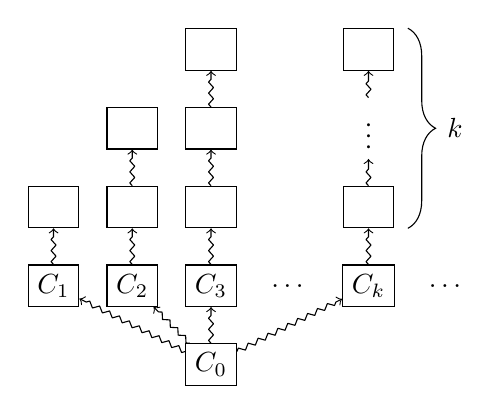
\begin{tikzpicture}
\node[draw] (c0) at (3,0) {$C_0$};
\node[draw] (c21) at (1,1) {$C_1$};
\node[draw] (c22) at (1,2) {\phantom{$C_0$}};
\node[draw] (c31) at (2,1) {$C_2$};
\node[draw] (c32) at (2,2) {\phantom{$C_0$}};
\node[draw] (c33) at (2,3) {\phantom{$C_0$}};
\node[draw] (c11) at (3,1) {$C_3$};
\node[draw] (c12) at (3,2) {\phantom{$C_0$}};
\node[draw] (c13) at (3,3) {\phantom{$C_0$}};
\node[draw] (c14) at (3,4) {\phantom{$C_0$}};
\node             at (4,1) {$\dots$};
\node[draw] (c41) at (5,1) {$C_k$};
\node[draw] (c42) at (5,2) {\phantom{$C_0$}};
\node       (c43) at (5,3) {$\vdots$};
\node[draw] (c44) at (5,4) {\phantom{$C_0$}};
\node             at (6,1) {$\dots$};
\draw[line join=round,
decorate, ->,decoration={
    zigzag,
    segment length=4,
    amplitude=.9,post=lineto,
    post length=2pt
}] (c0) -- (c21);
\draw[line join=round,
decorate, ->,decoration={
    zigzag,
    segment length=4,
    amplitude=.9,post=lineto,
    post length=2pt
}] (c21) -- (c22);
\draw[line join=round,
decorate, ->,decoration={
    zigzag,
    segment length=4,
    amplitude=.9,post=lineto,
    post length=2pt
}] (c0) -- (c31);
\draw[line join=round,
decorate, ->,decoration={
    zigzag,
    segment length=4,
    amplitude=.9,post=lineto,
    post length=2pt
}] (c31) -- (c32);
\draw[line join=round,
decorate, ->,decoration={
    zigzag,
    segment length=4,
    amplitude=.9,post=lineto,
    post length=2pt
}] (c32) -- (c33);
\draw[line join=round,
decorate, ->,decoration={
    zigzag,
    segment length=4,
    amplitude=.9,post=lineto,
    post length=2pt
}] (c0) -- (c11);
\draw[line join=round,
decorate, ->,decoration={
    zigzag,
    segment length=4,
    amplitude=.9,post=lineto,
    post length=2pt
}] (c11) -- (c12);
\draw[line join=round,
decorate, ->,decoration={
    zigzag,
    segment length=4,
    amplitude=.9,post=lineto,
    post length=2pt
}] (c12) -- (c13);
\draw[line join=round,
decorate, ->,decoration={
    zigzag,
    segment length=4,
    amplitude=.9,post=lineto,
    post length=2pt
}] (c13) -- (c14);
\draw[line join=round,
decorate, ->,decoration={
    zigzag,
    segment length=4,
    amplitude=.9,post=lineto,
    post length=2pt
}] (c0) -- (c41);
\draw[line join=round,
decorate, ->,decoration={
    zigzag,
    segment length=4,
    amplitude=.9,post=lineto,
    post length=2pt
}] (c41) -- (c42);
\draw[line join=round,
decorate, ->,decoration={
    zigzag,
    segment length=4,
    amplitude=.9,post=lineto,
    post length=2pt
}] (c42) -- (c43);
\draw[line join=round,
decorate, ->,decoration={
    zigzag,
    segment length=4,
    amplitude=.9,post=lineto,
    post length=2pt
}] (c43) -- (c44);
\draw[decorate,decoration={brace,amplitude=10pt}]
([xshift=5mm]c44.north) -- ([xshift=5mm]c42.south) node [black,midway,xshift=6mm] {$k$};
\end{tikzpicture}
\]
The $k$th approximant contains configurations whose traces all
terminate in fewer than $k$ steps. No approximant can contain
configuration $C_0$, since there is no bound $k$ on the length of its
traces. Yet this configuration will be admitted by a total correctness
specification whose postcondition is $\mathit{true}$, since it is the
case that each of its traces terminates.

Therefore, in the presence of infinite branching, the fixed point
characterisations of total correctness must be weakened to an
implication. Preservation of greatest lower bounds is unaffected by
infinite branching, so the characterisation of partial correctness
remains intact.

\begin{eqnarray*}
\seqspec{P}c{Q} & ~⇔~ & (\{c\}×P) ⊆ νX\ldotp \SafeOne_Q(X) \\
\totalspec{P}c{Q} & ~⇐~ & (\{c\}×P) ⊆ μX\ldotp \SafeOne_Q(X) 
\end{eqnarray*}

\section{Related work}
\label{sec:related}

Clarke~\cite{clarke79} was the first to study the correspondence
between greatest/least fixed points and partial/total correctness. He
remarks that
\begin{quote}the fixedpoints of $Γ$ form a complete lattice under the
natural partial ordering on $\pow(\State)$. The top element of this
lattice is the weakest precondition for partial correctness and the
bottom element is the weakest precondition for total
correctness.~\cite[p.~279]{clarke79}
\end{quote} 
%
We note three ways in which the current work extends on Clarke's
original observation. First, Clarke's work is in the setting of a
particular programming language that provides syntax for sequencing,
conditionals, assignment and recursive calls to parameterless
procedures. In this paper, we need not tackle issues of programming
language syntax, since we work at the level of arbitrary transition
systems. Second, Clarke's work is in the setting of a big-step
semantics; that is, the meaning of each programming construct maps an
initial state directly to a final state. We work with a small-step
semantics (as described by a transition system), which means that our
approach handles parallel programs without any further work. Big-step
semantics is well-known to be unable to handle parallelism, as
acknowledged by Clarke, who remarks that he `[is] currently attempting
to extend this fixedpoint theory to additional programming features
such as parallelism'~\cite[p.~292]{clarke79}. The definition of total
correctness in a small-step setting requires more nuance than in a
big-step setting, where it is trivial. Third, Clarke's work applies
only in a deterministic setting: a program has either a single final
state, or none at all. We allow for highly non-deterministic programs,
and only restrict the amount of non-determinism in the case of total
correctness.

Recent work on various Hoare logics for concurrency have used (mildly
disguised) greatest fixed point calculations to obtain a partial
correctness semantics. See, for example,
\cite[Definition~3.2]{vafeiadis11} and
\cite[Definition~25]{dinsdale-young+13}. The result in this paper
could prove helpful when those program logics are extended to total
correctness.

Jacobs and Gries have proposed \emph{general correctness} as a way to
unify partial and total correctness~\cite{jacobs+85}. It would be
interesting to investigate whether general correctness can be also
characterised as a fixed point calculation.

The idea of using the least and greatest fixed point of the same
function has been previously exploited by
Paulson~\cite[\S3]{paulson97a}, who obtains the set of finite lists
from a function's least fixed point, and the set of possibly-infinite
(`lazy') lists from its greatest fixed point.

\paragraph{Acknowledgements} This work was supported by EPSRC grant
EP/K011499/1. I would like to thank Edmund Clarke, Alastair Donaldson,
Tony Hoare, Peter Lammich, and Andreas Lochbihler for helpful feedback
and discussions.

\bibliographystyle{abbrv}
\bibliography{/Users/jpw48/Dropbox/John}


\end{document}